\chapter{Đọc thêm: Mô hình CAPM và Đo lường Hiệu suất (Dahlquist \& Knight)}
\label{ch:M3L2-reading1}

% Nguồn: Dahlquist, Julie, and Rainford Knight. "Principles of Finance." OpenStax, 2022.
% Phần cần đọc: Section 15.3 (The Capital Asset Pricing Model) & 15.4 (Applications in Performance Measurement)
% Nội dung bắt buộc đọc: được kiểm tra trong mọi bài đánh giá (kể cả Quiz).

\section{Thông tin nguồn}

\begin{itemize}
  \item \textbf{Nguồn:} Dahlquist, Julie, and Rainford Knight. \emph{Principles of Finance}. OpenStax Press, 2022. (truy cập mở tại \url{https://openstax.org/details/books/principles-finance})
  \item \textbf{Phần cần đọc:} Section 15.3: The Capital Asset Pricing Model (CAPM); Section 15.4: Applications in Performance Measurement
\end{itemize}

\section{15.3 Mô hình Định giá Tài sản Vốn (CAPM)}

\subsection*{Mục tiêu học tập}
Sau khi hoàn thành mục này, bạn sẽ có thể:
\begin{itemize}
  \item Định nghĩa phần bù rủi ro (risk premium).
  \item Giải thích khái niệm beta.
  \item Tính lợi suất yêu cầu của một chứng khoán bằng CAPM.
\end{itemize}

\subsection*{Lãi suất Phi rủi ro}

Mô hình định giá tài sản vốn (capital asset pricing model, CAPM) là một lý thuyết tài chính dựa trên ý tưởng rằng nhà đầu tư sẵn sàng nắm giữ cổ phiếu có rủi ro hệ thống cao hơn nên được thưởng nhiều hơn khi chấp nhận rủi ro thị trường này. CAPM tập trung vào rủi ro hệ thống, thay vì rủi ro riêng của từng cổ phiếu, vì rủi ro đặc thù doanh nghiệp có thể loại bỏ thông qua đa dạng hóa.

Giả sử ông bà bạn tặng bạn \$20,000. Sau khi tốt nghiệp đại học, bạn dự định đi làm vài năm rồi nộp đơn vào trường luật. Bạn muốn dùng \$20,000 ông bà cho để trả một phần học phí trường luật. Sẽ mất vài năm trước khi bạn sẵn sàng tiêu số tiền đó, và bạn muốn giữ nó an toàn. Đồng thời, bạn muốn đầu tư số tiền và để nó tăng trưởng cho đến khi bạn sẵn sàng vào trường luật.

Mặc dù bạn muốn kiếm lợi suất trên số tiền để có nhiều hơn \$20,000 vào lúc bắt đầu trường luật, mục tiêu chính của bạn là giữ tiền an toàn. Bạn đang tìm một khoản đầu tư phi rủi ro. Cho chính phủ Mỹ vay tiền được coi là khoản đầu tư rủi ro thấp nhất bạn có thể thực hiện. Bạn có thể mua một chứng khoán Kho bạc Mỹ. Khả năng chính phủ Mỹ không trả được nợ gần như bằng 0. Mặc dù về lý thuyết, không khoản đầu tư nào an toàn 100\%, đầu tư vào chứng khoán chính phủ Mỹ nhìn chung được coi là một khoản đầu tư phi rủi ro vì rủi ro cực kỳ nhỏ.

Lãi suất bạn có thể kiếm được bằng cách mua chứng khoán Kho bạc Mỹ là một đại diện cho lãi suất phi rủi ro. Nó được dùng làm chuẩn đầu tư. Lãi suất trung bình cho tín phiếu Kho bạc Mỹ 3 tháng từ 1928 đến 2020 là 3.36\%. Bạn có thể thấy rằng bạn sẽ không trở nên giàu có nhờ đầu tư vào tín phiếu Kho bạc Mỹ. Tuy nhiên, một đặc điểm khác của chứng khoán Kho bạc Mỹ là độ biến động của chúng có xu hướng thấp hơn nhiều so với cổ phiếu. Thực tế, độ lệch chuẩn của lợi suất tín phiếu Kho bạc Mỹ là 3.0\%. Khác với lợi suất cổ phiếu, lợi suất tín phiếu Kho bạc Mỹ chưa bao giờ âm. Lợi suất hàng năm thấp nhất là 0.03\%, xảy ra vào năm 2014.

\subsection*{Phần bù Rủi ro}

Bạn biết rằng nếu dùng \$20,000 để đầu tư vào cổ phiếu thay vì tín phiếu Kho bạc Mỹ, kết quả đầu tư sẽ không chắc chắn. Khoản đầu tư của bạn có thể sinh lời tốt, nhưng cũng có rủi ro mất tiền. Bạn sẽ chỉ sẵn sàng chấp nhận rủi ro này nếu được đền bù xứng đáng. Nói cách khác, bạn sẽ chỉ sẵn sàng chấp nhận rủi ro đầu tư vào cổ phiếu nếu bạn nghĩ rằng làm vậy sẽ mang lại nhiều tiền hơn so với đầu tư vào chứng khoán Kho bạc Mỹ.

Từ 1928 đến 2020, lợi suất trung bình của chỉ số cổ phiếu S\&P 500 là 11.64\%, cao hơn nhiều so với lợi suất trung bình 3.36\% của tín phiếu Kho bạc Mỹ. Tuy nhiên, lợi suất cổ phiếu, với độ lệch chuẩn 19.49\%, cũng biến động nhiều hơn nhiều. Thực tế, có 25 năm mà lợi suất của chỉ số S\&P 500 âm.

Bạn có thể không muốn chấp nhận rủi ro mất một phần số tiền ông bà đã cho vì bạn đang để dành nó cho trường luật. Nếu vậy, bạn sẽ muốn đầu tư vào chứng khoán Kho bạc Mỹ. Bạn có thể có tiền để dành cho các mục tiêu dài hạn khác, như nghỉ hưu, mà bạn sẵn sàng chấp nhận một số rủi ro. Lợi suất thêm mà bạn kiếm được khi chấp nhận rủi ro được gọi là phần bù rủi ro (risk premium). Phần bù rủi ro có thể được hiểu là phần thưởng cho việc bạn sẵn sàng gánh chịu rủi ro.

Phần bù rủi ro được tính bằng chênh lệch giữa lợi suất bạn nhận được khi chấp nhận rủi ro và lợi suất bạn sẽ nhận được nếu không chấp nhận rủi ro. Dùng lợi suất trung bình của S\&P 500 (để đo những gì nhà đầu tư chấp nhận rủi ro kiếm được) và lãi suất tín phiếu Kho bạc Mỹ (để đo những gì nhà đầu tư không chấp nhận rủi ro kiếm được), phần bù rủi ro được tính là:

$$
\text{Phần bù rủi ro} = 11.64\% - 3.36\% = 8.28\%
$$

\subsection*{Beta}

Phần bù rủi ro đại diện cho mức một nhà đầu tư nắm giữ danh mục thị trường được thưởng cho rủi ro. Nhà đầu tư mua một cổ phiếu, ví dụ DAL, trải nghiệm độ biến động, được đo bằng độ lệch chuẩn của lợi suất cổ phiếu đó. Hãy nhớ rằng một phần độ biến động đó, độ biến động gây ra bởi rủi ro đặc thù doanh nghiệp, có thể được loại bỏ thông qua đa dạng hóa. Vì nhà đầu tư có thể loại bỏ rủi ro đặc thù doanh nghiệp thông qua đa dạng hóa, họ sẽ không được thưởng cho rủi ro đó. Nhà đầu tư được thưởng cho lượng rủi ro hệ thống họ gánh chịu.

\subsection*{Diễn giải Beta}

Rủi ro liên quan đối với nhà đầu tư là rủi ro hệ thống họ gánh chịu. Rủi ro hệ thống của một cổ phiếu cụ thể được đo bằng mức độ cổ phiếu đó di chuyển cùng thị trường. Thước đo mức độ một cổ phiếu di chuyển cùng thị trường được gọi là beta của nó. Một cổ phiếu có xu hướng di chuyển đồng bộ với thị trường sẽ có beta bằng 1. Với các cổ phiếu này, nếu thị trường tăng 10\%, cổ phiếu nhìn chung cũng tăng 10\%; nếu thị trường giảm 5\%, cổ phiếu có beta bằng 1 cũng có xu hướng giảm 5\%.

Nếu một công ty có beta lớn hơn 1, cổ phiếu có xu hướng di chuyển mạnh hơn theo cùng hướng với thị trường. Ví dụ, nếu một cổ phiếu có beta bằng 2, cổ phiếu sẽ có xu hướng tăng 20\% khi thị trường tăng 10\%. Nếu thị trường giảm 5\%, cùng cổ phiếu đó sẽ có xu hướng giảm gấp đôi, tức 10\%. Do đó, cổ phiếu có beta lớn hơn 1 trải qua biến động lớn hơn thị trường chung và được coi là rủi ro hơn cổ phiếu trung bình.

Mặt khác, cổ phiếu có beta nhỏ hơn 1 trải qua biến động nhỏ hơn thị trường chung. Ví dụ, beta bằng 0.5 nghĩa là cổ phiếu có xu hướng biến động chỉ bằng 50\% biến động thị trường chung. Vậy, nếu thị trường tăng 10\%, cổ phiếu có beta 0.5 sẽ có xu hướng tăng chỉ 5\%. Thị trường giảm 5\% sẽ có xu hướng gắn với mức giảm 2.5\% của cổ phiếu.

\subsection*{Tính Beta}

Phép tính beta cho DAL được minh họa trong Hình 15.3. Lợi suất hàng tháng của DAL và S\&P 500 được vẽ trên biểu đồ. Mỗi điểm trong biểu đồ phân tán tương ứng với một tháng từ 2018 đến 2020; ví dụ, điểm nằm xa nhất ở góc trên bên phải đại diện cho tháng 11/2020. Lợi suất của S\&P 500 tháng đó là 10.88\%; lợi suất này được vẽ trên trục ngang. Lợi suất của DAL trong tháng 11/2020 là 31.36\%; lợi suất này được vẽ trên trục dọc.

Bạn có thể thấy rằng nhìn chung, khi toàn bộ thị trường chứng khoán đo bằng S\&P 500 dương, lợi suất của DAL cũng dương. Tương tự, trong các tháng mà lợi suất S\&P 500 âm, lợi suất của DAL cũng thường âm. Vẽ một đường khớp nhất với dữ liệu, còn gọi là đường hồi quy, tóm tắt mối quan hệ giữa lợi suất của DAL và S\&P 500. Độ dốc của đường này, 1.39, chính là beta của DAL. Beta đo lượng rủi ro hệ thống mà DAL có.

\begin{figure}[H]
\centering
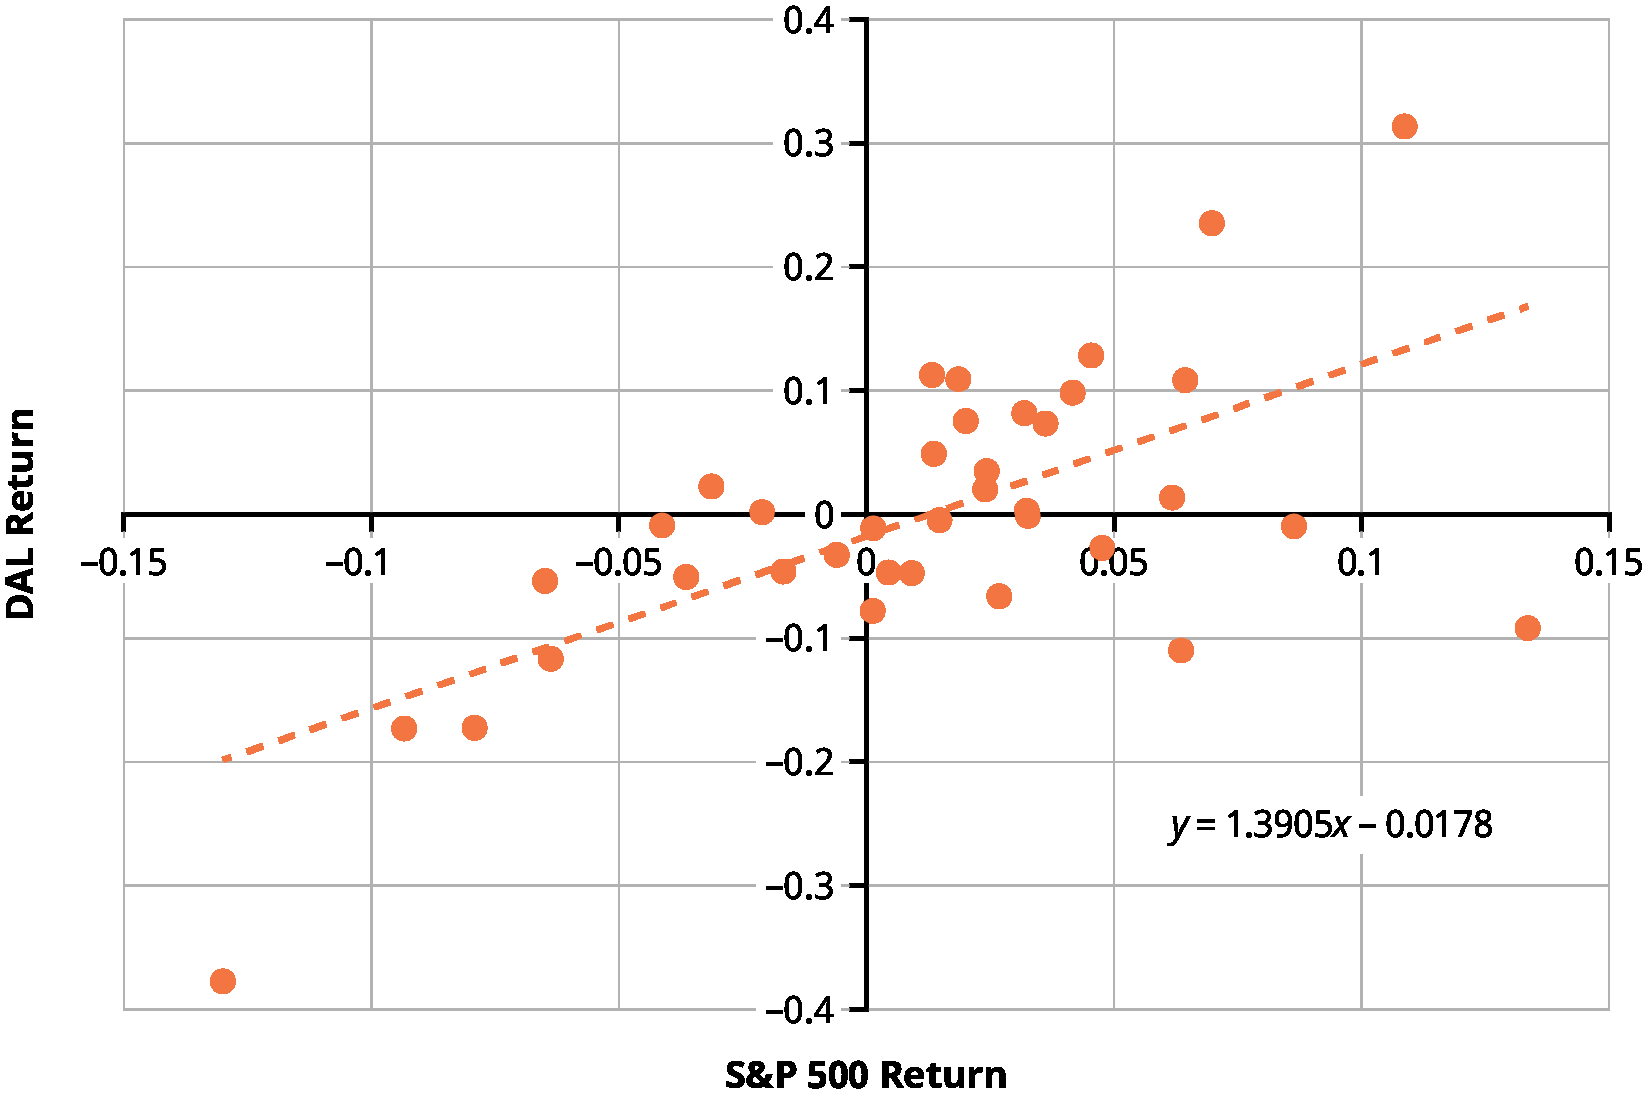
\includegraphics[width=0.7\linewidth]{gfx/m3l2_dahlquist_fig15-3_beta_calc.png}
\par\smallskip{\small \textbf{Hình 15.3:} Tính Beta cho DAL (nguồn dữ liệu: Yahoo! Finance)}
\end{figure}

\subsection*{Công thức CAPM}

Vì beta 1.39 của DAL lớn hơn 1, DAL rủi ro hơn cổ phiếu trung bình trên thị trường. Lý thuyết tài chính cho thấy nhà đầu tư mua DAL sẽ kỳ vọng một tỷ lệ lợi suất cao hơn để đền bù cho rủi ro này. DAL có 139\% rủi ro hệ thống của cổ phiếu trung bình; do đó, nhà đầu tư vào cổ phiếu này nên nhận 139\% phần bù rủi ro thị trường.

Công thức mô hình định giá tài sản vốn (CAPM) là

$$
R_e = R_f + \beta (R_m - R_f)
$$

trong đó $R_e$ là lợi suất kỳ vọng của tài sản, $R_f$ là lãi suất phi rủi ro, và $R_m$ là lợi suất kỳ vọng của thị trường. Với lợi suất trung bình S\&P 500 là 11.64\% và lợi suất trung bình tín phiếu Kho bạc Mỹ là 3.36\%, lợi suất kỳ vọng của DAL sẽ được tính là:

$$
R_e = 3.36\% + 1.39 \times (11.64\% - 3.36\%) = 14.87\%
$$

\begin{framed}
\textbf{LIÊN KẾT ĐẾN VIỆC HỌC: Tính Beta}

Nhiều nhà cung cấp dữ liệu cổ phiếu và thông tin đầu tư sẽ liệt kê beta của một công ty. Các nguồn khác nhau có thể không đưa ra cùng một giá trị beta cho một công ty. Ví dụ, vào đầu tháng 2/2021, Yahoo! Finance báo cáo beta của DAL là 1.46, trong khi MarketWatch báo cáo là 1.29. Cả hai con số này đều hơi khác so với 1.39 tính được trong biểu đồ ở trên.

Có một số lý do khiến beta có thể hơi khác nhau giữa các nguồn. Một là khung thời gian dùng trong phép tính beta. Dữ liệu ba năm được dùng để tính beta trong Hình 15.3. Khung thời gian từ ba đến năm năm thường được dùng khi tính beta. Một lý do khác khiến các nguồn khác nhau có thể báo cáo beta khác nhau là tần suất thu thập dữ liệu. Lợi suất hàng tháng được dùng trong Hình 15.3; một số nhà phân tích sẽ dùng dữ liệu hàng tuần. Cuối cùng, S\&P 500 được dùng để đo lợi suất thị trường trong Hình 15.3; S\&P 500 là một trong những thước đo phổ biến nhất về lợi suất thị trường chung, nhưng vẫn có các lựa chọn thay thế được một số nhà phân tích sử dụng.
\end{framed}

\section{15.4 Ứng dụng trong Đo lường Hiệu suất}

\subsection*{Mục tiêu học tập}
Sau khi hoàn thành mục này, bạn sẽ có thể:
\begin{itemize}
  \item Diễn giải tỷ số Sharpe.
  \item Diễn giải phép đo Treynor.
  \item Diễn giải alpha Jensen.
\end{itemize}

\subsection*{Tỷ số Sharpe}

Nhà đầu tư muốn một thước đo về mức độ giỏi của một nhà quản lý tiền chuyên nghiệp trước khi giao phó số tiền khó nhọc kiếm được của mình cho người đó đầu tư. Giả sử bạn thấy một quảng cáo trong đó McKinley Investment Management tuyên bố rằng danh mục của khách hàng họ có lợi suất trung bình 20\% mỗi năm. Bạn biết rằng lợi suất trung bình hàng năm này vô nghĩa nếu không biết thêm về mức độ rủi ro của chiến lược công ty. Trong mục này, ta xem xét một số cách đánh giá mức độ rủi ro của một chiến lược đầu tư.

Một thước đo cơ bản về hiệu suất đầu tư có điều chỉnh rủi ro là tỷ số Sharpe. Tỷ số Sharpe được tính bằng phần bù rủi ro của danh mục chia cho độ lệch chuẩn của lợi suất danh mục, dùng công thức:

$$
\text{Sharpe Ratio} = \frac{R_P - R_f}{\sigma_P}
$$

Phần bù rủi ro của danh mục là lợi suất danh mục $R_P$ trừ lợi suất phi rủi ro $R_f$; đây là phần thưởng cơ bản cho việc gánh chịu rủi ro. Nếu lợi suất phi rủi ro là 3\%, khách hàng của McKinley Investment Management kiếm được 20\% trên danh mục của họ có lợi suất vượt trội 17\%.

Độ lệch chuẩn của lợi suất danh mục, $\sigma_P$, là một thước đo rủi ro. Mặc dù bạn thấy khách hàng của McKinley kiếm được lợi suất trung bình khá tốt là 20\%, bạn nhận ra lợi suất rất biến động. Trong một số năm, khách hàng kiếm được nhiều hơn 20\%, và trong các năm khác, lợi suất thấp hơn nhiều, thậm chí âm. Độ biến động đó dẫn đến độ lệch chuẩn của lợi suất là 26\%. Tỷ số Sharpe sẽ là $17\%/26\% = 0.65$.

Như vậy, tỷ số Sharpe có thể được hiểu là tỷ số phần thưởng trên rủi ro. Độ lệch chuẩn ở mẫu số có thể được hiểu là đơn vị rủi ro mà nhà đầu tư gánh chịu. Tử số là phần thưởng nhà đầu tư nhận được khi chấp nhận rủi ro đó.

\begin{framed}
\textbf{LIÊN KẾT ĐẾN VIỆC HỌC: Tỷ số Sharpe}

Tỷ số Sharpe được phát triển bởi người đạt giải Nobel William F. Sharpe. Bạn có thể truy cập trang web của Sharpe tại Đại học Stanford để tìm các video trong đó ông thảo luận về các chủ đề tài chính và liên kết đến nghiên cứu của ông cũng như lời khuyên của ông về cách đầu tư.
\end{framed}

\subsection*{Phép đo Hiệu suất Treynor}

Một thước đo tỷ số phần thưởng trên rủi ro khác về hiệu suất đầu tư là tỷ số Treynor. Tỷ số Treynor được tính là:

$$
\text{Treynor Ratio} = \frac{R_P - R_f}{\beta_P}
$$

Cũng như tỷ số Sharpe, tử số của tỷ số Treynor là phần bù rủi ro của danh mục; điểm khác biệt là tỷ số Treynor tập trung vào rủi ro hệ thống, dùng beta của danh mục ở mẫu số, trong khi tỷ số Sharpe tập trung vào tổng rủi ro, dùng độ lệch chuẩn của lợi suất danh mục ở mẫu số.

Nếu McKinley Investment Management có một danh mục với lợi suất 20\% trong năm năm qua, với beta 1.2 và lãi suất phi rủi ro 3\%, tỷ số Treynor sẽ là:

$$
\text{Treynor Ratio} = \frac{20\% - 3\%}{1.2} = 14.17\%
$$

Cả tỷ số Sharpe và Treynor đều là thước đo tương đối về hiệu suất đầu tư, nghĩa là không có một con số tuyệt đối cho biết hiệu suất đầu tư là tốt hay xấu. Hiệu suất của một nhà quản lý đầu tư phải được xem xét trong tương quan với các nhà quản lý khác hoặc với một chỉ số chuẩn tham chiếu.

\subsection*{Alpha Jensen}

Alpha Jensen là một thước đo phổ biến khác về hiệu suất đầu tư. Nó được tính bằng lợi suất danh mục thô trừ đi lợi suất danh mục kỳ vọng dự đoán bởi CAPM:

$$
\alpha = R_P - \left[ R_f + \beta_P (R_m - R_f) \right]
$$

Giả sử lợi suất thị trường trung bình là 12\%. Alpha Jensen sẽ là bao nhiêu cho danh mục của McKinley Investment Management với lợi suất trung bình 20\% và beta 1.2?

$$
\alpha = 20\% - \left[ 3\% + 1.2 \times (12\% - 3\%) \right] = 20\% - 13.8\% = 6.2\%
$$

Khác với tỷ số Sharpe và Treynor, vốn có ý nghĩa theo nghĩa tương đối, alpha Jensen có ý nghĩa theo nghĩa tuyệt đối. Alpha bằng 0.062 cho thấy danh mục McKinley Investment Management mang lại lợi suất cao hơn 6.2\% so với kỳ vọng dựa trên mức độ rủi ro của danh mục. Alpha dương cho thấy danh mục có lợi suất bất thường (abnormal return). Nếu alpha Jensen bằng 0, lợi suất danh mục đúng bằng những gì được kỳ vọng dựa trên mức độ rủi ro của danh mục đo bằng beta.

\begin{framed}
\textbf{THỰC HÀNH: So sánh Lợi suất và Rủi ro của các Danh mục}

Bạn đang phỏng vấn hai nhà quản lý đầu tư. Ông Wong cho thấy lợi suất trung bình trên danh mục của ông trong 10 năm qua là 14\%, với độ lệch chuẩn 8\% và beta 1.2. Bà Petrov cho thấy lợi suất trung bình trên danh mục của bà trong 10 năm qua là 16\%, với độ lệch chuẩn 10\% và beta 1.6. Bạn biết rằng trong 10 năm qua, lãi suất chứng khoán Kho bạc Mỹ trung bình là 2\% và lợi suất S\&P 500 trung bình là 11\%. Bạn nghĩ nhà quản lý danh mục nào đã làm tốt hơn?

\textbf{Lời giải:}

Tỷ số Sharpe cho danh mục của ông Wong là $(14\%-2\%)/8\% = 1.5$, và tỷ số Treynor là $(14\%-2\%)/1.2 = 10\%$. Tỷ số Sharpe cho danh mục của bà Petrov là $(16\%-2\%)/10\% = 1.4$, và tỷ số Treynor là $(16\%-2\%)/1.6 = 8.75\%$.

Alpha Jensen cho danh mục của ông Wong là $14\% - [2\% + 1.2\times(11\%-2\%)] = 1.2\%$.

Alpha Jensen cho danh mục của bà Petrov là $16\% - [2\% + 1.6\times(11\%-2\%)] = -0.4\%$.

Cả ba thước đo hiệu suất danh mục đều cho thấy danh mục của ông Wong hoạt động tốt hơn danh mục của bà Petrov. Mặc dù bà Petrov có lợi suất trung bình lớn hơn, danh mục bà quản lý lại rủi ro hơn. Danh mục của bà Petrov biến động hơn danh mục của ông Wong, dẫn đến độ lệch chuẩn cao hơn. Danh mục của bà Petrov có beta cao hơn, nghĩa là nó có lượng rủi ro hệ thống cao hơn. CAPM cho thấy một danh mục với beta 1.6 nên có lợi suất kỳ vọng 16.4\%. Vì danh mục của bà Petrov có lợi suất trung bình thấp hơn mức đó, nhà đầu tư vào danh mục của bà Petrov không được đền bù cho rủi ro họ đã chấp nhận nhiều như kỳ vọng.
\end{framed}
